
%(BEGIN_QUESTION)
% Copyright 2010, Tony R. Kuphaldt, released under the Creative Commons Attribution License (v 1.0)
% This means you may do almost anything with this work of mine, so long as you give me proper credit

Every instrument has at least one input and at least one output.  For instruments responding linearly, the correspondence between input and output is proportional:

$$\includegraphics[width=15.5cm]{i04545x01.eps}$$

A practical example of this is a pressure transmitter, in this case one with an input range of 0 to 1023 PSI and an output of 4-20 mA:

$$\includegraphics[width=15.5cm]{i04545x02.eps}$$

If you happened to measure an output current of 14.7 mA from this pressure transmitter, it would be a simple matter for you to calculate the corresponding input pressure to be 684.13 PSI.

\vskip 10pt

However, students are often taken by surprise when they encounter an analog-to-digital converter (ADC) or digital-to-analog converter (DAC) and are asked to correlate input and output for such devices.  What might seem a daunting task at first, though, soon reveals itself to be the same input-to-output correspondence calculations they've seen all along in the guise of analog sensors and other instruments.

Take for example this analog-to-digital converter, with a 10-bit output (a ``count'' range of 0 to 1023) and a 4-20 mA input:

$$\includegraphics[width=15.5cm]{i04545x03.eps}$$

Calculate the corresponding ``count'' output of this ADC circuit given a 6.82 mA input signal.

\underbar{file i04545}
%(END_QUESTION)





%(BEGIN_ANSWER)

Count = 180 (rounding low) or 181 (rounding high)

%(END_ANSWER)





%(BEGIN_NOTES)

First, converting the given 6.82 mA input value into a per-unit figure:

$${6.82 \hbox{ mA} - 4 \hbox{ mA} \over 20 \hbox{ mA} - 4 \hbox{ mA}} = 0.17625 \hbox{ per unit}$$

We know that this is a 10-bit converter, therefore its count range (expressed in decimal) must be 0 to 1023 counts.  Thus, we may multiply the 0.17625 per-unit figure by the maximum count value of 1023 to see how many counts this ADC will output at 6.82 mA:

\vskip 10pt

$$(0.17625)(1023 \hbox{ counts}) = 180.30375 \hbox{ counts}$$

\vskip 10pt

Since we don't know anything about how this particular ADC digitizes the signal, we cannot predict whether the output will be rounded up, rounded down, or perhaps even ``bobble'' between the upper and lower rounded values:

\vskip 10pt

Output ``count'' value = 180 or 181

%INDEX% Electronics review: ADC resolution

%(END_NOTES)


